\chapter{Power Flow in an Electromagnetic Wave}\label{lec:lec27}
\definecolor{lightblue}{RGB}{173,216,230}
\begin{mdframed}[backgroundcolor=lightblue, linewidth=1pt,  hidealllines=true]
\section{Objective}
\begin{enumerate}
	\item To understand the power flow associated with electromagnetic fields from Maxwell's equations
	\item The importance of poynting factors in power flow
\end{enumerate}
\end{mdframed}
	\subsection{INTRODUCTION}
Up till now, we have seen that a time-varying electric and magnetic field constitutes a wave phenomenon. Thus this wave requires some power or energy to flow. In this chapter, we look at the power flow associated with electromagnetic waves. We do some derivation starting with Maxwell's Equation and find out the power flow associated with a time-varying electromagnetic field.

 We have also investigated a wave which is called uniform plane wave i.e. a wave propagation in an unbound medium. However, in developing the power flow equations associated with electromagnetic waves, we would do a general analysis and not restrict our focus to uniform plane waves, at the end we find out the power flow associated with uniform plane waves which we have discussed in \autoref{lec:lec25} and \autoref{lec:lec26}. So whenever we are at the beginning of analysis in electromagnetics, we go back to Maxwell's Equations and find answers that are consistent with Maxwell's equation. The same thing we do have if we are asked the question,  \emph{``What power do we get for the power flow associated with an electromagnetic field?"}

From Maxwell's Equation, we have;
\begin{align}
\nabla\times\bar{E}=-\frac{\delta\bar{B}}{\delta t} \cdot 
\end{align} 
If the permeability of the system is not a function of time,
\begin{align}
\vec{B}=\mu \vec{H}\\
\frac{\delta\bar{B}}{\delta t}= -\mu\frac{\delta\bar{H}}{\delta t}
\end{align}
Therefore;
\begin{align}
\nabla\times\bar{E} = -\mu \frac{\delta\bar{H}}{\delta t} 
\end{align} 
and similarly, if permittivity  $(\epsilon) $ is not a function of time,
\begin{align}
\vec{D} = \epsilon \vec{E}\\
\nabla\times\bar{H} =\bar{J} + \frac{\delta\bar{D}}{\delta t}  =  J + \epsilon\frac{\delta\bar{E}}{\delta t} 
\end{align}

We start with these two basic equations and then try to investigate the power flow associated with electric and magnetic fields. We essentially make use of the vector identities and then try to find out the meaning of some expressions we would get from using the vector identities.

Recall,
\begin{align}
\nabla \cdot ( \bar{A}\times\bar{C} ) = C \cdot (\nabla\times\bar{A}) - \bar{A}\cdot(\nabla\times\bar{C})
\label{eqn:vectoridentity} 
\end{align} 
For arbitrary vectors $\bar{A}$ and $\bar{C}$,

Let $\bar{A}$ be the electric field $\bar{E}$ and $ \bar{C} $ be the Magnetic Field $\bar{H}$, substituting for $\bar{A}$ as $\bar{E}$ and $\bar{C}$ as $\bar{H}$ into equation\ref{eqn:vectoridentity}, we have;
\begin{align}
\nabla\cdot(\bar{E}\times\bar{H})= \bar{H}\cdot(\nabla\times\bar{E})-\bar{E}\cdot(\nabla\times\bar{H})
\end{align} 
Now Substituting for $\nabla\times\bar{E}$ and $\nabla\times\bar{H}$, we have;
\begin{align}
\nabla\cdot(\bar{E}\times\bar{H})=
\bar{H}\cdot(-\mu\frac{\delta\bar{H}}{\delta t}) - \bar{E}\cdot(\bar{J}+\epsilon\frac{\delta\bar{E}}{\delta t})
\label{eqn:enhpowflow}
\end{align}
Recall from vector identities, we  have that;

\begin{dmath*}
\frac{\delta}{\delta t}(\bar{A}\cdot\bar{C})= \bar{A}\cdot\frac{\delta\bar{C}}{\delta t}+\bar{C}\cdot\frac{\delta\bar{A}}{\delta t} 
\frac{\delta}{\delta t}(\bar{A}\cdot\bar{A})
= \bar{A}\cdot\frac{\delta\bar{A}}{\delta t}+\bar{A}\cdot\frac{\delta\bar{A}}{\delta t}
= 2\bar{A}\cdot\frac{\delta A}{\delta t}
\end{dmath*}
Making $\bar{A}\cdot\frac{\delta A}{\delta t} $ the subject of formula,
we have;
\begin{dmath}
\bar{A}\cdot\frac{\delta\bar{A}}{\delta t}=\frac{1}{2}\frac{\delta}{\delta t}(\bar{A}\cdot\bar{A})=\frac{1}{2}\frac{\delta}{\delta t} |A|^{2}
\label{eqn:vectoridentity2} 
\end{dmath}
Having refreshed ourselves with these identities, we can deduce from equation\ref{eqn:enhpowflow}, that;
\begin{dmath*}
\nabla\cdot(\bar{E}\times\bar{H}) = -\mu\left(\bar{H}\cdot\frac{\delta\bar{H}}{\delta t}\right) - \bar{E}\cdot\bar{J} - \epsilon\left(\bar{E}\cdot\frac{\delta\bar{E}}{\delta t}\right)
\end{dmath*}
Therefore, relating equation\ref{eqn:vectoridentity2}, to equation\ref{eqn:enhpowflow}, we have;
\begin{dmath}
\nabla\cdot(\bar{E}\times\bar{H})=-\frac{\mu}{2}\frac{\delta}{\delta t}|\bar{H}|^{2} -  \frac{\epsilon}{2}\frac{\delta}{\delta t}|\bar{E}|^{2}-\bar{E}\cdot\bar{J} 
\end{dmath}
We can investigate this expression over a closed surface or volume to have some meaning associated with these quantities.
\begin{dmath*}
\iiint_{v}\nabla\cdot(\bar{E}\times\bar{H})dv  = \iiint_v-\frac{\mu}{2}\frac{\delta}{\delta t}|\bar{H}|^{2}dv-
\iiint_{v}\frac{\epsilon}{2}\frac{\delta}{\delta t}|\bar{E}|^{2}dv -\iiint_{v}\bar{E}\cdot\bar{J}dv 
\end{dmath*}
If we assume that the volume enclosed is not varying as a function of time i.e. fixed volume, that is to say, that the field varies with time but space does not vary with time. We can take $\frac{\delta}{\delta t}$ out of the integration and apply the divergence theorem on $ \int_{v}\nabla\cdot(\bar{E}\times\bar{H}) $ to convert it to a closed surface integral.

Thus,
\begin{dmath}
\oint(\bar{E}\times\bar{H})\cdot\bar{d}a  =  -\frac{\delta}{\delta t}  \int_{v}\frac{\mu}{2}|\bar{H}|^{2}dv -  \frac{\delta}{\delta t}\int_{v}\frac{\epsilon}{2}|\bar{E}|^{2}dv  -  \int_{v}\bar{E}\cdot\bar{J}dv 
\end{dmath}
We now substitute $ \bar{J}=\sigma\bar{E}, $ into $\bar{E}\cdot\bar{J}$ to get; 
$\bar{E}\cdot\bar{J}=\bar{E}\cdot\sigma\bar{E}=\sigma\bar{E}\cdot\bar{E}=\sigma|\bar{E}|^{2}$.

So,
\begin{dmath}
\oint(\bar{E}\times\bar{H})\cdot\bar{d}a = -  \frac{\delta}{\delta t}\int_{v} \frac{\mu}{2}|\bar{H}|^{2}dv -  \frac{\delta}{\delta t}\int_{v}\frac{\epsilon}{2}|\bar{E}|^{2}dv
- \int_{v}\sigma|\bar{E}|^{2}dv 
\end{dmath}
Each term in the above expression has a physical significance.

$\int_{v} \frac{\mu}{2}|\bar{H}|^{2}dv$ represents the total magnetic energy stored in the volume V hence the term $-\frac{\delta}{\delta t}\int_{v} \frac{\mu}{2}|\bar{H}|^{2}dv$ gives the rate of change of magnetic energy stored in the volume(The negative sign indicates a decrease).

Similarly, $\int_{v}\frac{\epsilon}{2}|\bar{E}|^{2}dv$ represents the total electrical energy stored in volume V hence the term $-\frac{\delta}{\delta t}\int_{v}\frac{\epsilon}{2}|\bar{E}|^{2}dv$ gives the rate of change of electrical energy stored in the volume(Again the negative sign indicates a decrease).

While the term $-\int_{v}\sigma|\bar{E}|^{2}dv $ represents the total ohmic loss in the volume due to the finite conductivity of the medium.

So if we have an amount of energy enclosed in a surface, these 3 total losses combined must be equal to the total outward energy going out from the closed surface (s). Since there is no other mechanism for energy consumption, from the law of conservation of energy, we get that $ \oint(\bar{E}\times\bar{H})\cdot\bar{da} $ must represent the net flow of energy coming out from the closed surface. So $ \oint(\bar{E}\times\bar{H})\cdot\bar{d}a $ (the net power outflow from a closed surface)  gives the net power flow of the electric and magnetic field from that closed surface. This is called \textbf{Poynting theorem}\footnote{
John Henry Poynting (Born 9, September 1852 and died 30, March 1914). He was an English physicist. He was a professor of physics at Mason Science College, from 1880 to 1900, and then at the successor institution, the University of Birmingham until his death.

He is known for the Poynting vector, Poynting Effect, Poynting's theorem 
Poynting was the youngest son of Thomas Elford Poynting, a Unitarian minister
}\index{poynting theroem}poynting theroem. 
\section{Poynting theorem and Poynting vector}
The \index{Poynting}Poynting theorem states that the cross-product of electric and magnetic fields integrated over a closed surface gives the total power flow from the closed surface. Now we have seen the quantity which represents the total power flow, then $\bar{E}\times\bar{H}$ is essentially the power density on the surface. So that when this power density is integrated over an area, it gives the total power flow from that surface area.
It should be kept in mind that, even though $ \oint(\bar{E}\times\bar{H})\cdot\bar{da} $ gives the net power flow from a closed surface, saying that $\bar{E}\cross\bar{H}$ should give the power density at any point on the surface, is only an arbitrary definition. The theorem does not state that $\bar{E}\cross\bar{H}$ gives the power density (or power flow per unit area) on the surface. Rather it states that the total power flows out of a closed surface is given by $ \oint(\bar{E}\times\bar{H})\cdot\bar{da} $. So saying $\bar{E}\cross\bar{H}$ is the power density which is true for every point on the surface of a sphere(due to symmetry), might not be true in some other cases.

Hence, it is arbitrary we take power density from here. It so happens that most of the time in practice, this arbitrary definition gives the power density correctly. But, it should be said that, if knowing $\bar{E}\times\bar{H}$, one already knows the power density at every point on the surface of the volume, this statement is not correct. There are many special cases where $\bar{E}\times\bar{H}$  may give power flow where there is no power flow at that point. So while using $\bar{E}\times\bar{H}$  as power density, one should be very careful. In most practical situations, however, the arbitrary definition that $\bar{E}\times\bar{H}$  gives power density at any location normally is valid.

So we have an important quantity called a power flow density $ \bar{P}=\bar{E}\times\bar{H} $ where $  \bar{P}  $ is called a POYNTING VECTOR\index{poynting vector}poynting vector for these fields. Poynting vector is an important concept in the electromagnetic wave as it tells the power flow associated with any particular point in space and also tells in which direction the power is flowing. The first thing we note here is that if you have an electric and magnetic field, the Poynting vector is the direction perpendicular to both $ \bar{E} $ and  $ \bar{H} $. So if $  \bar{P}  $  has to be non-zero in terms of power flow, then $ \bar{E} $ and  $ \bar{H} $ should not be parallel to each other. In a case where  $ \bar{E} $ and  $ \bar{H} $ are parallel to each other, then  $ \bar{E}\times\bar{H} $=0 and this connotes that there will be no net power flow associated with this. So only when the component of the electric and magnetic fields are perpendicular to each other would they contribute to power flow and the direction of power flow is perpendicular to $ \bar{E} $ and  $ \bar{H} $    fields. It should be noted that for us to have a power flow, $ \bar{E} $ and  $ \bar{H} $  must cross each other. Whenever $ \bar{E} $ and  $ \bar{H} $ cross each other, there is a possibility of power flow. We use the word possibility here because this quantity   $ \bar{E}\times\bar{H} $ is telling you the so-called instantaneous power if we know the values of  $ \bar{E} $ and  $ \bar{H} $. At that instant of time at some point in space, we can always find out $ \bar{E}\times\bar{H} $ and we get $  \bar{P}  $ which will give the Poynting vector at that instant of time. It is possible that even if $  \bar{P}  $ is finite at some instance of time, there may be no net power flow over long periods. That is in time average sense, there may not be power flow associated with that system. So Poynting Vector $  \bar{P}  $ which we defined as $ \bar{E}\times\bar{H} $  serves the purpose of defining the power flow. But in Practical Systems, a more useful quantity would be the time average value of the Poynting Vector, because the Poynting vector at some instant of time may be negative and that is like getting negative power. Of course, when dealing with space, we can say negative power flow means direction change. All these complications come in simply if we use $ \bar{E}\times\bar{H} $ to get  $  \bar{P}  $ since $  \bar{P}  $  can be positive or negative and $  \bar{P}  $  can be a complex quantity too if there is a phase difference between $ \bar{E} $ and  $ \bar{H} $ with time. So what we do is, we try to get the time average value of the Poynting vector and it is a much more useful quantity for finding out if there is a net flow of power associated with the Electric and Magnetic fields. 

As we have seen earlier, we are interested only in the analysis of time-harmonic fields, so we assume that the electric and magnetic fields are varying sinusoidally as a function of time. The only thing now is when there is a phase difference between $ \bar{E} $ and  $ \bar{H} $, we then ask what is the average power flow associated with $ \bar{E} $ and  $ \bar{H} $ in that case.

Now we define the general time-varying electric and magnetic fields which vary as a function of space and time as;

$ \bar{E}=\bar{E_0} e^{\jmath\omega t+j\phi_{e}}$,
$ \bar{H}=\bar{H_0} e^{\jmath\omega t+j\phi_{h}}$.
We take the unit vector associated with $ \bar{E_0} $ and  $ \bar{H_0} $ as $ \hat{e} $ and $ \hat{h} $, so we remember that we are only taking either the real or the imaginary part of $ e^{\jmath\omega t} $ for simple analysis. It doesn't mean $ \bar{E} $ cannot be complex. But for simplicity,
$ \bar{E}=\mathfrak{Re}(E_0e^{\jmath\omega t}e^{j\phi e} )\cdot\hat{e} $   
$ \bar{H}=\mathfrak{Re}(H_0e^{\jmath\omega t}e^{j\phi h} )\cdot\hat{h} $ 
where  $ \hat{e} $ and $ \hat{h} $ 
gives the unit vector of the electric and magnetic field, $ \phi_{e} $ and $ \phi_{h} $ are the phases of the electric and magnetic fields and $ E_0 $ and  $ H_0 $ are the amplitude of the electric and magnetic fields. So the real parts give an instantaneous value of the electric and magnetic field. Once this is known, we can find the Poynting vector at that instant in time.
\begin{align*}
\bar{E}(t)=E_0\cos(\omega t+\phi_{e})\hat{e}\\ 
\bar{H}(t)=H_0\cos(\omega t+\phi_{h})\hat{h}
\end{align*}
The power flow density at that instant t is the Poynting vector  $ \bar{P} $  would be;
\begin{dmath*}
\bar{P}=\bar{E}\times\bar{H} = E_0H_0\cos(\omega t+\phi_{e}) \cos(\omega t+\phi_{h}) (\hat{e}\times\hat{h}) =  \frac{E_0H_0}{2} (\cos(\phi_{e}-\phi_{h})+\cos(2\omega t + \phi_{e}+\phi_{h}))  (\hat{e}\times\hat{h}) 
\end{dmath*}
How did we get to the last expression, we will see below. From compound angle formulas, we have
\begin{dmath*}
\cos(\omega t+\omega t) =\cos\omega t\cos\omega t-\sin\omega t\sin\omega t =\cos^{2}\omega t-\sin^{2}\omega t=\cos^{2}\omega t-(1-\cos^{2}\omega t)
\end{dmath*}
Simplifying further, we get $ 2\cos^{2}\omega t-1 = \cos(2\omega t) $ or $ \cos^{2}\omega t=\frac{\cos^{2}\omega t+1}{2}$.

\begin{dmath*}
\sin(\omega t+\omega t) =\sin\omega t\cos\omega t+\cos\omega t\sin\omega t
\end{dmath*}
Simplifying further, we get $ 2\sin\omega t\cos\omega t$ or $  \sin\omega t\cos\omega t = \frac{\sin2\omega t}{2}$
\begin{dmath*}
\bar{P}= \bar{E}\times\bar{H}=E_0H_0\cos(\omega t+\phi_{e})\cos(\omega t+\phi_{h})\hat{e}\times\hat{h} 
= E_0H_0[(\cos\omega t\cos\phi_{e}-\sin\omega t\sin\phi_{e})(\cos\omega t\cos\phi_{h}-\sin\omega t\sin\phi_{h})]\hat{e}\times\hat{h} 
=  E_0H_0[\cos^{2}\omega t\cos\phi_{e}\cos\phi_{h}-\cos\omega t\sin\omega t\cos\phi_{e}\sin\phi_{h}-\cos\omega t\sin\omega t\sin\phi_{e}\cos\phi_{h}+\sin^{2}\omega t\sin\phi_{e}\sin\phi_{h}]\hat{e}\times\hat{h}
=E_0H_0[\cos^{2}\omega t\cos\phi_{e}\cos\phi_{h}+ ( 1 - \cos^{2}\omega t)\sin\phi_{e}\sin\phi_{h} -\cos\omega t\sin\omega t(cos\phi_{e}\sin\phi_{h} +\sin \phi_{e}\cos\phi_{h})]\hat{e}\times\hat{h} 
=E_0H_0[\cos^{2}\omega t(\cos\phi_{e}\cos\phi_{h}-\sin\phi_{e}\sin\phi_{h})+\sin\phi_{e}\sin\phi_{h}-\cos\omega t\sin\omega t(\cos\phi_{e}\sin\phi_{h}+\sin\phi_{e}\cos\phi_{h})] \hat{e}\times\hat{h} 
= E_0H_0[\cos^{2}\omega t\cos(\phi_{e}+\phi_{h})+\sin\phi_{e}\sin\phi_{h}-\cos\omega t\sin\omega t\sin(\phi_{e}+\phi_{h})      ]\hat{e}\times\hat{h}  
=E_0H_0 [(\frac{\cos2\omega t+1}{2})\cos(\phi_{e}+\phi_{h})+\sin\phi_{e}\sin\phi_{h}-\frac{\sin2\omega t}{2}\sin(\phi_{e}+\phi_{h})] \hat{e}\times\hat{h}  
=E_0H_0[\frac{\cos2\omega t\cos(\phi_{e}+\phi_{h})}{2}- \frac{\sin2\omega t\sin(\phi_{e}+\phi_{h})}{2}+\frac{1}{2}\cos(\phi_{e}+\phi_{h})+\sin\phi_{e}\sin\phi_{h}]\hat{e}\times\hat{h} 
=E_0H_0[\frac{1}{2}\cos(2\omega t+\phi_{e}+\phi_{h})+\frac{1}{2}\cos(\phi_{e}+\phi_{h})+\sin\phi_{e}\sin\phi_{h}]\hat{e}\times\hat{h} 
=E_0H_0[\frac{1}{2}\cos(2\omega t+\phi_{e}+\phi_{h})+\frac{1}{2}\cos\phi_{e}\cos_{h} -\frac{1}{2}\sin\phi_{e}\sin\phi_{h}+\sin\phi_{e}\sin\phi_{h}]\hat{e}\times\hat{h} 
=E_0H_0[\frac{1}{2}\cos(2\omega t+\phi_{e}+\phi_{h})+\frac{1}{2}\cos\phi_{e}\cos\phi_{h} +\frac{1}{2}\sin\phi_{e}\sin\phi_{h}]\hat{e}\times\hat{h}
=\frac{ E_0H_0}{2}[\cos(\phi_{e}-\phi_{h})+\cos(2\omega t+\phi_{e}+\phi_{h})]\hat{e}\times\hat{h} 
\end{dmath*}
So when we take an average of this throughout the signal then $\cos(2\omega t+\phi_{e}+\phi_{h})$ will go to zero. Positive area cancels negative area. It corresponds to a waveform having 2f as its frequency. So over a period corresponding to $ T=\frac{2\pi}{\omega} $ the time average $ \bar{P}_{av} $ is; $ \frac{1}{T}\int^{T}_{0}\bar{P}dt $ with $ T=\frac{2\pi}{\omega} $.
\begin{dmath*}
\bar{P}_{av}=\frac{1}{T}\int^{T}_{0} \frac{ E_0H_0}{2}\cos(\phi_{e}-\phi_{h})dt(\hat{e}\times\hat{h})  
\frac{E_0H_0}{2} \cos(\phi_{e}-\phi_{h})(\hat{e}\times\hat{h}) 
=\frac{1}{2} \mathfrak{Re}[(E_0e^{j\omega t+j\phi_{e}}\hat{e})\times(H_0e^{-j\omega t-j\phi_{h}}\hat{h})]
=\frac{1}{2} \mathfrak{Re}[(E_0e^{j\omega t+j\phi_{e}}\hat{e})\times(H_0e^{j\omega t+j\phi_{h}}\hat{h})^{*}]  
\end{dmath*}
\begin{flushright}
\begin{footnotesize}
the * above represents the conjugate.
\end{footnotesize}
\end{flushright} 
But Originally; $ \bar{E}=\bar{E_0}e^{j\omega t+j\phi_{e}}$ and $ H=\bar{H_0}e^{j\omega t+j\phi_{e}} $

We now have the average power to be; $\bar{P}_{av}=\mathfrak{Re}(\bar{E}\times\bar{H}^{*})$. This means that if we know the electric and magnetic field in complex forms(the electric and magnetic field may not be in the time phase), in general, we can calculate $ \bar{E}\times\bar{H}^{*} $. Taking half of the real part gives the average power flow which is associated with that electromagnetic wave. So $\bar{P}_{av}=\frac{1}{2}\mathfrak{Re}(\bar{E}\times\bar{H}^{*})$ is a real quantity. All these problems we had with instantaneous power flow, $ \bar{P}=\bar{E}\times\bar{H} $ complex depending on the phase between $ \bar{E} $ and $ \bar{H} $, have now been taken care of. This also implies that, the overall power flow which is associated with these fields at a particular location. It is possible that, at a particular location, the instantaneous Poynting vector might be negative or positive but the average power Poynting vector will always be positive and that gives the net power flow associated with these electric and magnetic fields.

This is the concept regularly used in finding out the average power flow associated with electromagnetic waves. So in determining average power flow, there are two things now essential. One is, $ \bar{E} $ and $ \bar{H} $ fields must be perpendicular (or have components perpendicular to each other), only then would we have a cross product which will be non-zero. Secondly, the electric and magnetic fields should not be in TIME QUADRATURE. This means the electric and magnetic fields should not differ by a phase of $90^{o}$. If this happens, $ \mathfrak{Re}(\bar{E}\times\bar{H}^{*})=0 $ and then we will not have any real power flow associated with the fields at that point. So in general it is possible that if you take the electric and magnetic fields, you get a complex power. The real part of the quantity gives the net power flow at that location and the imaginary part (j conjugate ) gives the power oscillating around that point. So at some instant in time, the power might be going in a certain direction, and after some time, the power will be coming back in the same direction. So the imaginary part of $ E\times\bar{H}^{*} $ gives the oscillatory power called the REACTIVE POWER. Whereas the real part gives the net power flow or the RESISTIVE POWER flow at the location. So the concept of the Poynting vector and the average Poynting vector is very important because by using this concept, we can calculate the net power flow at a particular location.

\section{Uniform Plane wave}\index{uniform plane wave}uniform plane wave
We can then apply this concept to a case of a uniform plane wave. So we may ask, \emph{how much power density does a uniform plane wave carry when it travels in a media?} In Uniform plane waves, electric and magnetic fields are perpendicular to each other. With $ \bar{E} $ and $ \bar{H} $ shown below
\begin{figure}[h]
\centering
\textsc{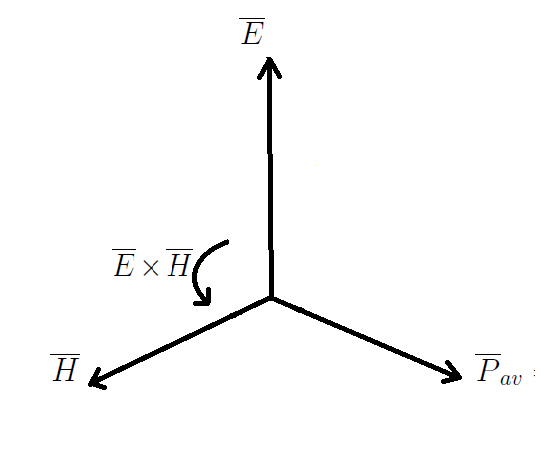
\includegraphics[width=.7\linewidth]{graphics/cc}}
\caption{Direction of power flow of an electromagnetic wave}
\end{figure}

The direction of power flow is given by the right-hand rule. $ \bar{E}\times\bar{H} $ as we realize has the direction of $ \bar{P}_{av} $ which is also the same as the direction of wave propagation. As we have seen in the case of a uniform plane wave, $ \bar{E} $, $ \bar{H} $ and the direction of \index{propagation}propagation are mutually perpendicular to each other. If we say the electric field is $ \bar{E}=E_0e^{-j\beta z}\hat{x} $ having phase variation in the Z direction, therefore;
$ \bar{H}=H_0e^{-j\beta z}\hat{y} $,
\begin{dmath*}
\bar{P}_{av}=\frac{1}{2}\mathfrak{Re}(\bar{E}\times\bar{H}^{*})
=\frac{1}{2}\mathfrak{Re}(E_0e^{-j\beta z}H_0e^{+j\beta z})(\hat{x}\times\hat{y})
=\frac{1}{2}\mathfrak{Re}(E_0H_0\hat{z})=\frac{1}{2}(E_0H_0\hat{z}) 
\end{dmath*}
So for a uniform plane wave, the average Poynting vector will be half $ E_0H_0 $ in direction $ \hat{z} $ with $ \bar{E} $ in $ \hat{x} $ and $ \bar{H} $ in $ \hat{y} $ direction.

Now we can take specific cases for the uniform plane wave in an unbound medium in which the wave is propagating. For a DIELECTRIC MEDIUM, $ \bar{E} $ and $ \bar{H} $ are related by the intrinsic impedance of the medium.
$ \frac{E}{H}=\eta $ = intrinsic impedance.

Assuming $H_{0} \text{ and } E_{0}$ are complex quantities, then $\bar{P}_{av}=\frac{1}{2} \mathfrak{Re}(E_0H_0^{*}\hat{z}) $. Substituting $\eta$ into $ \bar{P}_{av}=\frac{1}{2} \mathfrak{Re}(E_0H_0^{*}\hat{z}) $ and making it in terms of the electric field only,  we have;
\begin{dmath*}
\bar{P}_{av}=\frac{1}{2} \mathfrak{Re}\left\{E_0(\frac{E_0}{\eta})^{*}\right\}\hat{z}  
\end{dmath*}
This can also be written as $ \bar{P}_{av}= \frac{1}{2}\mathfrak{Re}\left\{\eta H_0(H_0^{*})\right\}\hat{z} $ in terms of magnetic field.

We now have that 
\begin{dmath*}
\bar{P}_{av}=\frac{1}{2}\mathfrak{Re}\left\{\frac{|E_0|^{2}}{\eta^{*}}\right\}\hat{z}
\end{dmath*}
or 
\begin{dmath}
\bar{P}_{av}=\frac{1}{2}\mathfrak{Re}\left\{\eta|H_0|^{2}\right\}\hat{z}
\end{dmath}
So from here, we can find the average power flow associated with a uniform plane wave in an unbound medium. For a dielectric medium,for which $ \eta=\sqrt{\frac{\mu}{2}} $, that is for an ideal dielectric, $ \eta $ is real.
$ \bar{P}_{av}=\frac{1}{2}\frac{|E_0|^{2}}{\eta} $ or $ \frac{1}{2}\eta|H_0|^{2} $. So in a dielectric medium, if we know the peak amplitude of either the electric or magnetic field, the permeability and permittivity of the medium, and then $ \eta $ which is real, we can get the power flow density associated with this uniform plane wave with above equations.

In general, if the medium has a finite conductivity that is non-zero or very large, then we use

$ \bar{P}_{av}=\mathfrak{Re}(\frac{|E_0|^{2}}{2\eta^{*}})\hat{z} $ or  $ \bar{P}_{av}= \frac{1}{2}\mathfrak{Re}\left\{\eta H_0(H_0^{*})\right\}\hat{z} $ 
as $ \eta $ is a complex quantity in this case.

For the extreme case of a good conductor, to get the average power, Recall;
\begin{dmath*}
\eta=\sqrt{\frac{\omega\mu}{2\sigma}}+j\sqrt{\frac{\omega\mu}{{2\sigma}}}
\end{dmath*}
Thus,
\begin{dmath*}
\bar{P}_{av}=\frac{1}{2}|E_0|^{2}\sqrt{\frac{\sigma}{2\omega\mu}} 
\end{dmath*}
that is because,
\begin{dmath*}
\bar{P}_{av}=\frac{1}{2}\mathfrak{Re}\left\{\frac{|E_0|^{2}}{\eta^{*}}\right\}=\frac{1}{2}\mathfrak{Re}\left\{\frac{|E_0|^{2}}{\sqrt{\frac{\omega\mu}{2\sigma}}-j\sqrt{\frac{\omega\mu}{\bar{2\sigma}}}}\right\}
\end{dmath*}
Finding the conjugate
\begin{dmath*}
\bar{P}_{av}= \frac{1}{2}\mathfrak{Re}\left\{\frac{|E_0|^{2}\left(\sqrt{\frac{\omega\mu}{2\sigma}}+j\sqrt{\frac{\omega\mu}{\bar{2\sigma}}}\right)}{\left(\sqrt{\frac{\omega\mu}{2\sigma}}-j\sqrt{\frac{\omega\mu}{\bar{2\sigma}}}\right)\left(\sqrt{\frac{\omega\mu}{2\sigma}}+j\sqrt{\frac{\omega\mu}{\bar{2\sigma}}}\right)}\right\}
\end{dmath*}
simplifying further,
\begin{dmath*}
\bar{P}_{av}=\frac{1}{2}\mathfrak{Re}\left\{\frac{|E_0|^{2}(\sqrt{\frac{\omega\mu}{2\sigma}}+j\sqrt{\frac{\omega\mu}{\bar{2\sigma}}})}{\frac{2\omega\mu}{2\sigma}}\right\}
= \frac{|E_0|^{2}}{2}\mathfrak{Re}\left\{\frac{\sigma}{\omega\mu}\left(\sqrt{\frac{\omega\mu}{2\sigma}}+j\sqrt{\frac{\omega\mu}{\bar{2\sigma}}}\right) \right\}
=\frac{|E_0|}{2}\frac{\sigma}{\omega\mu}\times\sqrt{\frac{\omega\mu}{2\sigma}}=\frac{1}{2}|E_0|^{2}\sqrt{\frac{\sigma}{2\omega\mu}} 
\end{dmath*}
Hence for a good conductor, we have, 
\begin{align}
\bar{P}_{av}=\frac{1}{2}|E_0|^{2}\sqrt{\frac{\sigma}{2\omega\mu}} 
\end{align}
So by using the concept of Poynting vector, we can find out the average power flow of any medium and at any particular location in space.

In the case of dielectric, it is straightforward because the intrinsic impedance is real. For a good conductor with finite conductivity, we go to the more general expression as the intrinsic impedance is complex.
\definecolor{lightblue}{RGB}{173,216,230}
\begin{mdframed}[backgroundcolor=lightblue, linewidth=1pt,  hidealllines=true]
\section{ExerciseList}
\begin{ExerciseList}
	\Exercise[label={ex11}] Explain the significance of Maxwell's Equations in the analysis of power flow associated with electromagnetic waves.
	\Exercise[label={ex11}] Derive the expressions for power flow in electromagnetic waves using Maxwell's Equations.
    \Exercise[label={ex11}] Define the Poynting vector and explain its significance in describing power flow associated with electromagnetic fields.
	\Exercise[label={ex11}] Discuss the conditions under which power flow occurs, considering the relationship between electric and magnetic fields.
	\Exercise[label={ex11}] Explain why time average power flow is considered more useful than instantaneous power flow in practical systems
	\Exercise[label={ex11}] Derive the expression for time average power flow associated with electric and magnetic fields in terms of the Poynting vector.
	\Exercise[label={ex11}] Discuss the power flow associated with a uniform plane wave in an unbound medium
	\Exercise[label={ex11}] Calculate the average power flow density for a dielectric medium and a good conductor, considering the intrinsic impedance.
	\Exercise[label={ex11}] Demonstrate how vector identities are applied to arrive at the expression 
	\(E \times H = -\mu\left(\frac{\partial}{\partial t} \lvert H \rvert^2\right) - 2\epsilon\left(\frac{\partial}{\partial t} \lvert E \rvert^2\right) - E \cdot J\)
	
	
\end{ExerciseList}
\end{mdframed}
